\documentclass[12pt]{article}
\usepackage{tikz}
\usetikzlibrary{arrows,shapes}
\usepackage{helvet}

% \setpagesize{width}{height}   {margin}
\newcommand{\setpagesize}[2]{
  \setlength{\pdfpagewidth}{#1}
  \setlength{\pdfpageheight}{#2}
  %\addtolength{\pdfpageheight}{#3}
  %\addtolength{\pdfpagewidth}{#3}
  \setlength{\textheight}{\pdfpageheight}
  \setlength{\textwidth}{\pdfpagewidth}
  %\setlength\topmargin{-1in}
  \setlength{\voffset}{-1in}
  \setlength{\topmargin}{0in}
  \setlength{\headheight}{0in}
  \setlength{\headsep}{0in}
  \setlength{\footskip}{0in}
  \setlength{\hoffset}{-1in}
  %\setlength{\oddsidemargin}{-1in}
  %\setlength{\evensidemargin}{-1in}
  \setlength{\oddsidemargin}{0in}
  \setlength{\evensidemargin}{0in}
  \setlength{\marginparwidth}{0in}
  \setlength{\marginparpush}{0in}
  \setlength{\marginparsep}{0in}
  \setlength{\parindent}{0in}
  \setlength{\parskip}{0in}
}



% pdftoppm -r 670 quad-2.pdf | pnmcrop -white | pnmpad -white -width 512 -height 512 | pnmtopng > quad.png

\newlength{\quadfigwidth}
\newlength{\quadfigheight}
\setlength{\quadfigwidth}{2cm}
\setlength{\quadfigheight}{2cm}

\setpagesize{\quadfigwidth}{\quadfigheight}

% 213, 74, 60
\definecolor{anred}{rgb}{0.83,0.29,0.24}

\addtolength{\voffset}{0.02\textheight}

\begin{document}
\thispagestyle{empty}

\centering
\def\star{}
\def\ticklen{1pt}
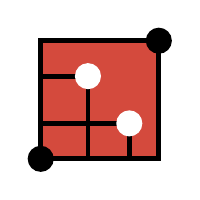
\begin{tikzpicture}[scale=1.5, line join=miter, line width=0.06cm]

	\tikzstyle{axes}=[]
    \def\cx{0.75}
    \def\cy{0.3}
    \def\dx{0.4}
    \def\dy{0.7}

    \draw [fill=anred] (0,0) -- (1,0) -- (1,1) -- (0,1) -- cycle;

	\draw (\cx,0) -- (\cx,\cy) -- (0,\cy);
   	\draw (\dx,0) -- (\dx,\dy) -- (0,\dy);

    \def\star{node{}}
    \begin{scope}[nodes={circle, radius=0.05, fill=black}]
      \draw
	  (0,0)     \star
	  (1,1)     \star;
    \end{scope}
    \begin{scope}[nodes={circle, radius=0.04, fill=white}]
      \draw
	  (\cx,\cy) \star
	  (\dx,\dy) \star;
    \end{scope}


  \end{tikzpicture}
\end{document}
